
\documentclass[landscape,norsk,11pt]{seminar} 
 
\def\everyslide{\sf}
\usepackage{babel}
\usepackage{ucs}
\usepackage[utf8x]{inputenc}

\usepackage[T1]{fontenc}

\usepackage{hyperref}
\usepackage{graphics}

\slideframe{none}

\title{Mo oažžut dihtora hálddašit lunddolaš giela válljenvejolašvuođaid giellaoahppanproseassas? -- Gielalaš ja pedagogalaš čuolmmat}

\author{Lene Antonsen, Biret Ánne Bals Baal\\
Saara Huhmarniemi, Trond Trosterud \\
 \scalebox{0.30}[0.30]{
\includegraphics{img/logoWeb070sh.jpg}}}
% \textit{http://giellatekno.uit.no/oahpa/}}
%  \scalebox{0.10}[0.10]{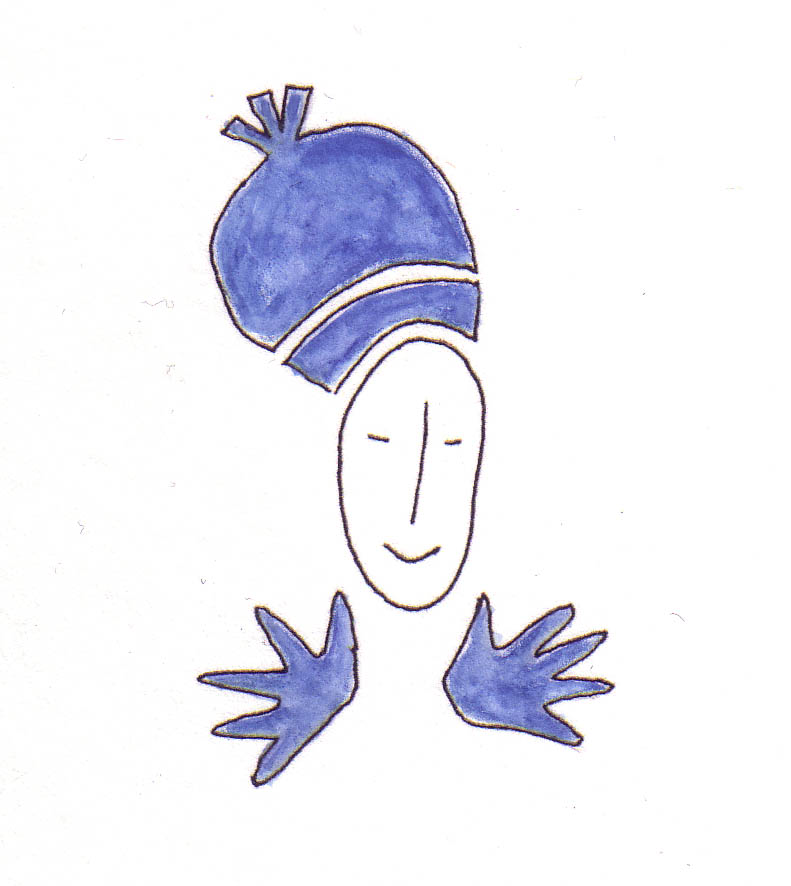
\includegraphics{img/vasta.png}} \\
\begin{document}
\begin{slide}

\maketitle


\newslide
\textit{http://giellatekno.uit.no/oahpa/}
\scalebox{0.30}[0.30]{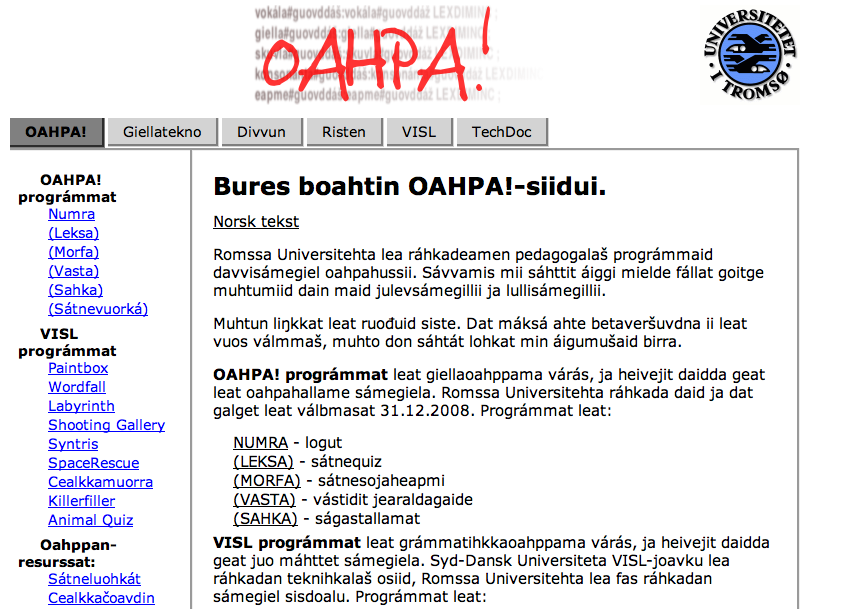
\includegraphics{img/gtoahpa.png}} 


\newslide
\textbf{VISL-prográmmat: oahppat grámmatihkka}\\
\newline
Sátneluohkáid, syntávssa\\


\newslide
\textbf{OAHPA-prográmmat: oahppat sámegiela}\\
\newline
\textbf{Leksa}: Sátnequiz - sámi/dáru ja dáru/sámi\\
\textbf{Numra}: Hárjehallat loguid\\
\textbf{Morfa}: Hárjehallat sojahit sániid, maid konteavsttas \\
\textbf{Vasta}: Hárjehallat vástidit jearaldagaide \\
\textbf{Sahka}: Hárjehallat ságastallat dihto fáttás

\newslide
\textit{http://victorio.uit.no/oahpa/morfa/}
\scalebox{0.35}[0.35]{
\includegraphics{img/oahpa.png}} 

\newslide
\textbf{Vasta}
\scalebox{0.90}[0.90]{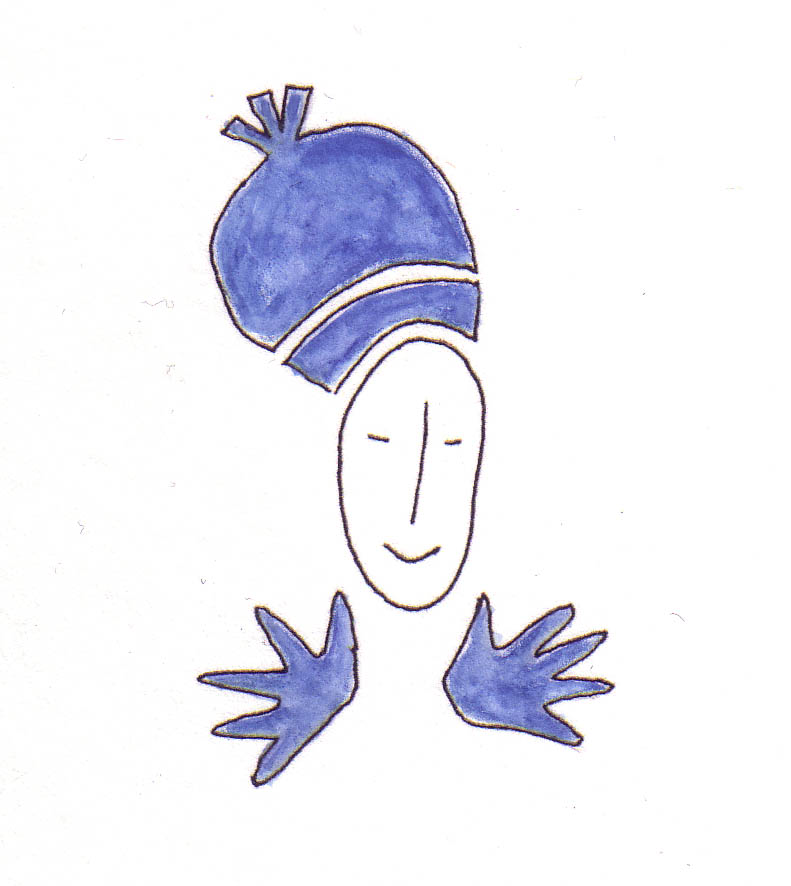
\includegraphics{img/vasta.png}} \\

%\newslide
%\textbf{Generating questions}
%\scalebox{.35}[.35]{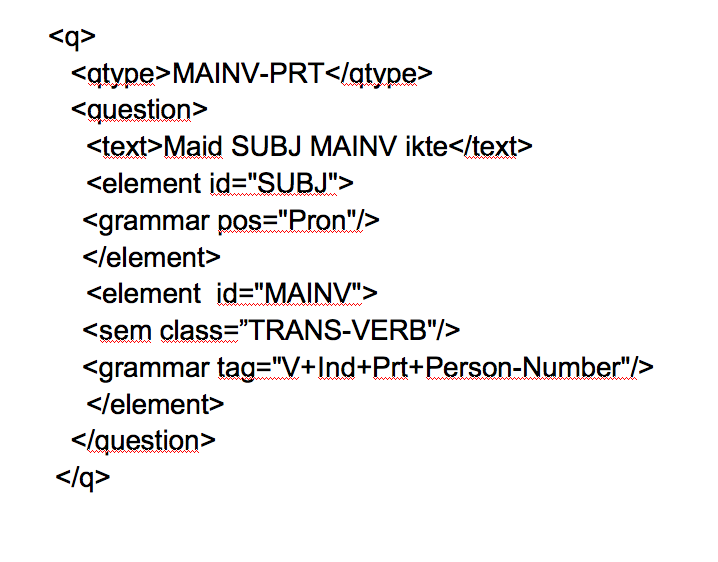
\includegraphics{img/xml_question.png}}

\newslide
\textbf{Pedagogalaš prográmmain dábálaččat ii leat giellateknologiija:} 
\begin{itemize}
\item multiple choice 
\item string -- omd. \textit{viesus} = 6 mearkka 
\end{itemize}

\textbf{Giellateknologiija:} \textit{viesus} = viessu N Sg Loc 


\newslide
\textbf{Áigumuš:}\\
Prográmma galgá bagadit studeantta seammá ládje go oahpaheaddji.

\newslide
\textbf{Omd.: "Maid don lohket ikte?"} \\
Dohkálaš vástádusat:
\begin{itemize}
\item Mun han lohken ollu \'aviissaid. 
\item Ikte mun gal lohken buori girjji. 
\item In lohkan maidege. 
\item Ikte in lohkan.
\end{itemize}

\newslide
\textbf{Maid don lohket ikte?}\\
Vasta bagada go vástádus ii leat dohkálaš:
\begin{itemize}
\item Mun lohket ollu \'aviissaid. --> Husk kongruens mellom subjekt og verbal.
\item Mun lohken ollu \'aviissat. --> Objektet skal være i akkusativ.
\item Don lohket ollu \'aviissat. --> Er du sikker på at du svarer i riktig person?
\end{itemize}

\newslide
\textbf{Mo mii dahkat dan?}\\
Govva min systemas

\newslide
Mii geavahit min máhtu:
\begin{itemize}
\item sámegiela syntávssa birra		
\item ohppiid gaskagiela birra
\end{itemize}


\newslide
\textbf{Lunddolaš ságastallan:} \\

\scalebox{0.40}[0.40]{
\includegraphics{img/lgiella1.png}} 

\newslide
\textbf{Lunddolaš ságastallan:} \\

\scalebox{0.40}[0.40]{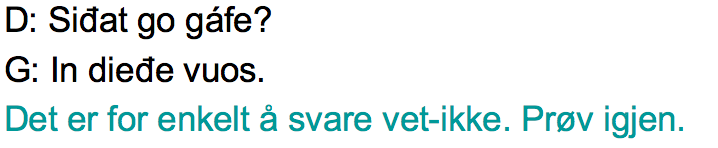
\includegraphics{img/lgiella2.png}} 

\newslide
\textbf{Lunddolaš ságastallan:} \\

\scalebox{0.40}[0.40]{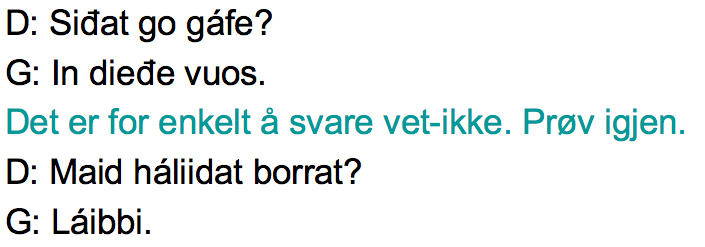
\includegraphics{img/lgiella3.png}} 
\newslide
\textbf{Lunddolaš ságastallan:} \\

\scalebox{0.40}[0.40]{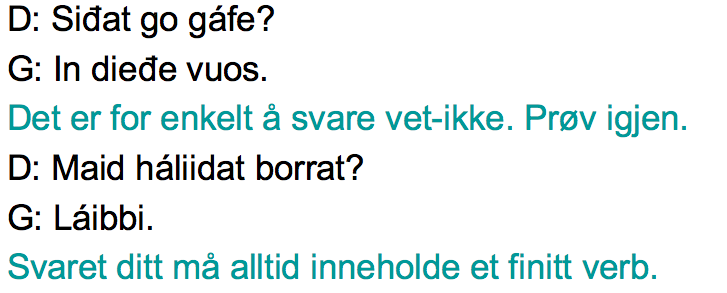
\includegraphics{img/lgiella4.png}} 
\newslide
\textbf{Lunddolaš ságastallan:} \\

\scalebox{0.40}[0.40]{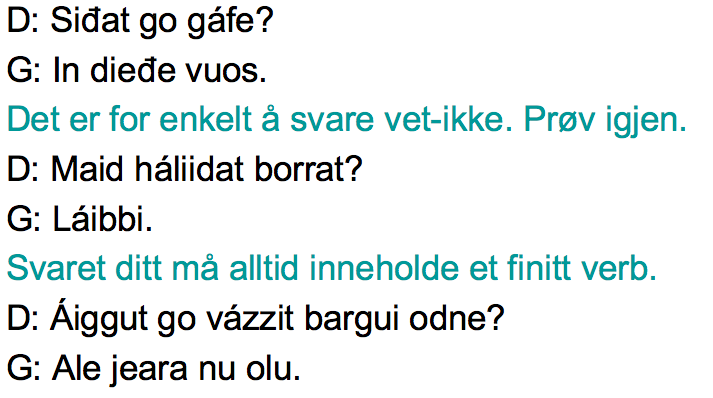
\includegraphics{img/lgiella5.png}} 
\newslide
\textbf{Lunddolaš ságastallan:} \\

\scalebox{0.40}[0.40]{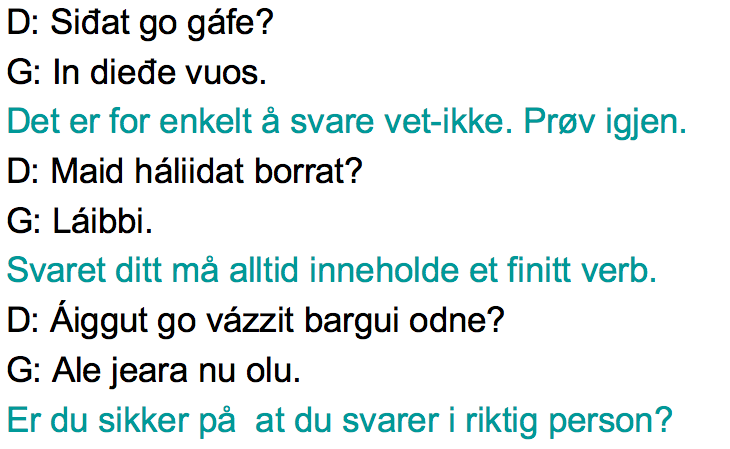
\includegraphics{img/lgiella6.png}} 


\newslide
\textbf{Didaktihkka versus pragmatihkka} \\
Mii háliidit geavaheaddji hárjehallat buot persovnnaid ja loguid. Dan dihte:
\begin{itemize}
\item{Ellipsa ii leat dohkálaš}
\item{Finihtta vearba lea bákkolaš}
\item{Ferte vástidit seammá vearbbain dalle go lea lunddolaš dan dahkat}
\item{Ii leat fátmmasteaddji 1. p duála ja plurála }
\item{\textit{In dieđe} ii leat dohkálaš vástádus}
\end{itemize}




\newslide
\textbf{Čuolmmat -- 1} \\
omd. cealkagis galgá leat dušše okta finihtta vearba: \\
\textit{*Mun áiggun vuolggán.}\\
\textit{Mun boran haman.}\\
-- finihtta-finihtta-konstrukšuvnnas vearbbain galgá leat seammá sojaheapmi\\
-- ii galgga leat advearba gaskkas

\newslide

LIST INFV =  astat ádjánit áigut álgit beassat berret bivvat boahtit ....

\newslide
\textbf{Čuolmmat -- 2: Nominatiiva versus akkusatiiva} \\
Eat sáhte luohttit sátneortnegii, ja subjeakta ii leat bákkolaš
\begin{itemize}
\item Jearaldat jearrá objeavtta (muhto lea muhtumin vejolaš vástidit objeavtta haga)
\end{itemize}
Geavahit semánttalaš seahtaid, omd: 
\begin{itemize}
\item vearbbaid bákkolaš argumeanttat - omd.  Strict Transitive Verbs
\item vearbbain ii sáhte leat HUMAN objeaktan? 
\end{itemize}

\newslide
\textbf{sáhttá go HUMAN leat objeaktan?} \\

 \textit{borrat}   - HUMAN sáhttá leat subjeakta, iige objeakta \\
  \textit{lohkat}  - seammá, muhto objeakta sáhttá leat namma, omd. Fosse


\newslide
\textbf{Čuolmmat -- 3: Áiggukeahtes lemma} \\
 
Omd.\textit{viessut}: \textit{viessut} Inf dahje \textit{viessat} Imprt \\
muhto mii árvidit ahte studeanta háliida čállit \textit{viesut}. \\
Vejolaš bálgát:

\begin{itemize}
\item{Váldit eret problemáhtalaš lemmaid dahje sátnehámiid}
\item{Jearrat geavaheaddjis, goappá don oaivvildat? \textit{viesut}  N dahje \textit{viessut} V }
\end{itemize}


\newslide
\textbf{Čuolmmat -- 4: sojaheamit dahket homonymiija} \\
omd. oamastangehčosat \\
\textit{biilas / biillas} \\
> Váldit eret oamastangehčosiid ?

> Kommenteret studentii ?\\
Mener du lokativ? I så fall er det feil stadieveksling.



%\newslide

%QA information retrieval how to process questions
%interactive, aske the user for clarification

%QA: 

%Question matrixes: generate a set of questions

%\newslide
%\textbf{Ovdamearka studeanttas}
%The output is manipulated  - it would not give two mappings to the same reading.
%\scalebox{.32}[.35]{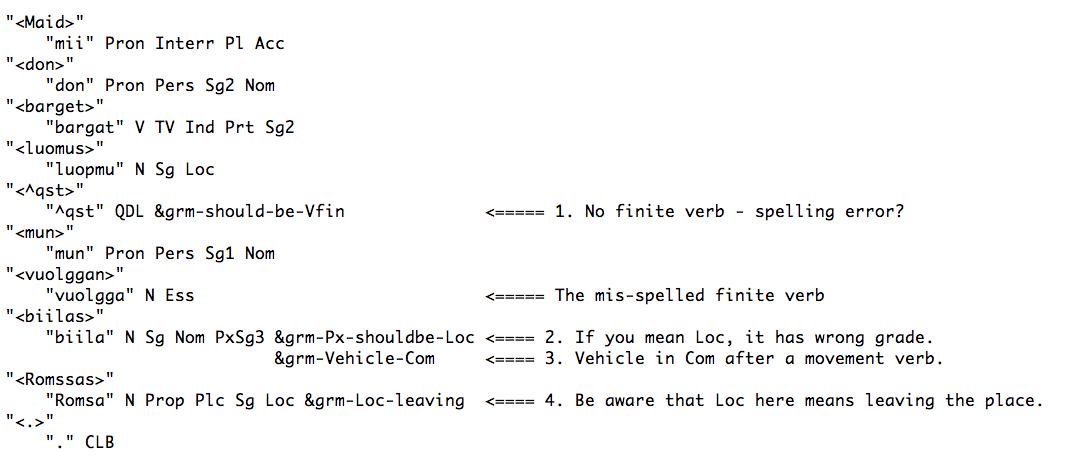
\includegraphics{img/sentence_example.png}}

\newslide
\textbf{Buoret ahte soames áššit báhcet divukeahttá go divvut dakkár mii leat riekta} \\
- muhto makkár vuorddámušat leat geavaheaddjis?

\newslide
\textbf{Evalueren ja buorideapmi}
\begin{itemize}
\item{Responsa geavaheddjiin}
\item{Responsa oahpaheddjiin}
\item{Logga neahtas}
\end{itemize}


\end{slide}
\end{document}




